\documentclass[sigconf]{acmart}

\newcommand{\FIXME}[1]{{\color{red}{\textbf{FIXME:}#1}}}

\usepackage{booktabs} % For formal tables

% Copyright
%\setcopyright{none}
%\setcopyright{acmcopyright}
%\setcopyright{acmlicensed}
\setcopyright{rightsretained}
%\setcopyright{usgov}
%\setcopyright{usgovmixed}
%\setcopyright{cagov}
%\setcopyright{cagovmixed}


% DOI
\acmDOI{10.475/123_4}

% ISBN
\acmISBN{123-4567-24-567/08/06}

%Conference
\acmConference[SHORTNAME'17]{ACM Long Conference Name conference}{July 1997}{City, State, Country} 
\acmYear{2017}
\copyrightyear{2017}

\acmPrice{15.00}

\usepackage{xspace}
\newcommand{\OurSys}{Wharf\xspace}

\begin{document}
\title{Mitigating faulty links using in-network computing}
%\title{SIG Proceedings Paper in LaTeX Format}
%\titlenote{Produces the permission block, and copyright information}
%\subtitle{Extended Abstract}

\author{Anirudh Chelluri \kern1em
 Andr\'e DeHon \kern1em
 Hans Giesen \kern1em
 Boon Thau Loo \kern1em
 Nishanth Prabhu \kern1em
 Lei Shi \kern1em
 John Sonchack \kern1em
 Nik Sultana}
\affiliation{%
\institution{University of Pennsylvania}}

%\author{Firstname Lastname}
%\authornote{Note}
%\orcid{1234-5678-9012}
%\affiliation{%
%  \institution{Affiliation}
%  \streetaddress{Address}
%  \city{City} 
%  \state{State} 
%  \postcode{Zipcode}
%}
%\email{email@domain.com}
%
%\author{Firstname Lastname}
%\orcid{1234-5678-9012}
%\affiliation{%
%  \institution{Affiliation}
%  \streetaddress{Address}
%  \city{City} 
%  \state{State} 
%  \postcode{Zipcode}
%}
%\email{email@domain.com}
%
%\author{Firstname Lastname}
%\orcid{1234-5678-9012}
%\affiliation{%
%  \institution{Affiliation}
%}
%\email{email@domain.com}
%
%\author{Firstname Lastname}
%\orcid{1234-5678-9012}
%\affiliation{%
%  \institution{Affiliation}
%}
%\email{email@domain.com}
%
%\author{Firstname Lastname}
%\orcid{1234-5678-9012}
%\affiliation{%
%  \institution{Affiliation}
%}
%\email{email@domain.com}


% The default list of authors is too long for headers}
%\renewcommand{\shortauthors}{F. Lastname et al.}
\renewcommand{\shortauthors}{A. Chelluri et al.}

\begin{abstract}
Failing network links are usually disabled, and packets are routed around them
until the links are repaired.  But it is often possible
to utilise some of a failing link's capacity. Losing what remains of a link's
capacity is deemed preferable to the erratic effect that unreliable links can
have on application-level behaviour.

We describe a new network function that relies on in-network computing to limit
the erratic effect of failing network links, to enable the continued use of
those links until they can be repaired. We argue that such a network function
can help mitigate rolling failures in datacenter networks, and that our design
can interoperate with existing network architecture and configuration choices,
such as for multi-path routing.

We model our design using ns-3, and evaluate our implementation on a physical
test-bed that includes programmable switches and reconfigurable hardware.
\end{abstract}

%
% The code below should be generated by the tool at
% http://dl.acm.org/ccs.cfm
% Please copy and paste the code instead of the example below. 
%
\begin{CCSXML}
<ccs2012>
 <concept>
  <concept_id>10010520.10010553.10010562</concept_id>
  <concept_desc>Computer systems organization~Embedded systems</concept_desc>
  <concept_significance>500</concept_significance>
 </concept>
 <concept>
  <concept_id>10010520.10010575.10010755</concept_id>
  <concept_desc>Computer systems organization~Redundancy</concept_desc>
  <concept_significance>300</concept_significance>
 </concept>
 <concept>
  <concept_id>10010520.10010553.10010554</concept_id>
  <concept_desc>Computer systems organization~Robotics</concept_desc>
  <concept_significance>100</concept_significance>
 </concept>
 <concept>
  <concept_id>10003033.10003083.10003095</concept_id>
  <concept_desc>Networks~Network reliability</concept_desc>
  <concept_significance>100</concept_significance>
 </concept>
</ccs2012>  
\end{CCSXML}

\ccsdesc[500]{Computer systems organization~Embedded systems}
\ccsdesc[300]{Computer systems organization~Redundancy}
\ccsdesc{Computer systems organization~Robotics}
\ccsdesc[100]{Networks~Network reliability}

% We no longer use \terms command
%\terms{Theory}

\keywords{ACM proceedings}


\maketitle

\section{Introduction}


\section{Background}
Fat-tree topology, and port density.
CorrOpt~\cite{Zhuo:2017:UMP:3098822.3098849}.

\section{Design}
For simplicity we assume that the underlying network is Ethernet, but this is
not a requirement.

\begin{figure}
  \centering
  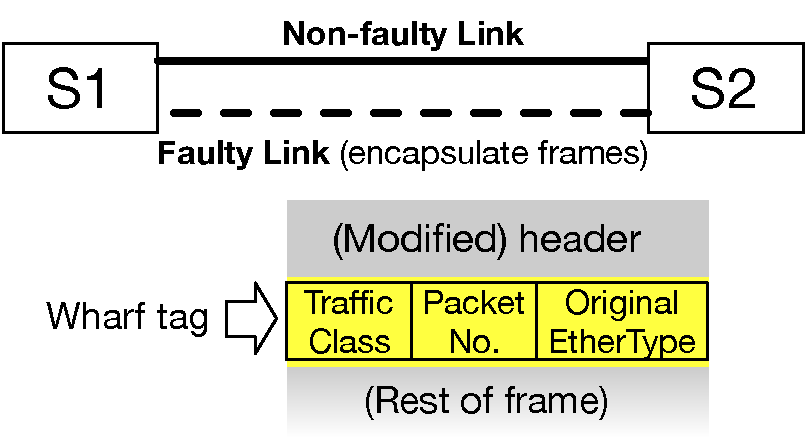
\includegraphics[width=0.4\paperwidth]{header_format.pdf}
  \caption{\label{fig:format}Switches can have multiple links between them.
  Traffic on faulty links is encapsulated as shown above: the frame's EtherType
  is moved inside the \OurSys tag (and later moved back after the frame crosses
  the link), the frame's EtherType is changed to \OurSys, and the packet is
  classified to a particular Traffic Class and given a transient link-local
  identifier.}
\end{figure}


\begin{figure}
  \centering
  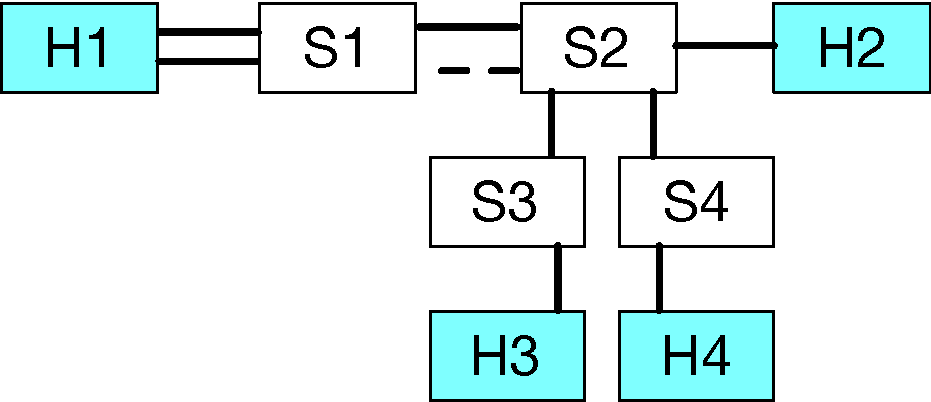
\includegraphics[width=0.3\paperwidth]{example_network.pdf}
  \caption{\label{fig:example-net}An example network consisting of four
  switches (S1-S4) and four hosts (H1-H4). Each link is assumed to have
  capacity $R$ unless the link is faulty, in which case it has capacity $F < R$.
  In this example, the failing link diminishes the bandwidth of H1.}
\end{figure}


\begin{figure}
  \centering
  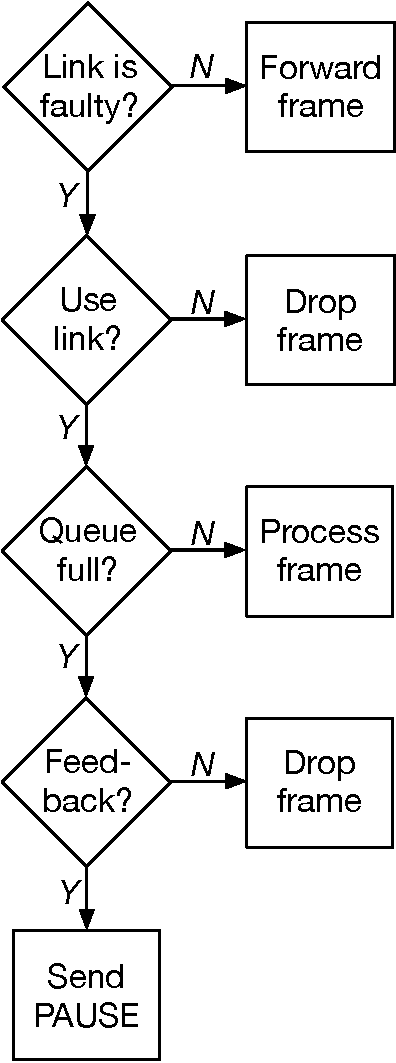
\includegraphics[width=0.2\paperwidth]{flowchart.pdf}
  \caption{\label{fig:flowchart}Outline of \OurSys's behaviour.}
\end{figure}


\section{Implementation}
\section{Evaluation}
\section{Conclusion}

\bibliographystyle{ACM-Reference-Format}
\bibliography{paper}

\end{document}
